\documentclass[conference]{IEEEtran}
\usepackage{graphicx}

% turn off hypenation
\tolerance=1
\emergencystretch=\maxdimen
\hyphenpenalty=10000
\hbadness=10000

\begin{document}

\title{Project Final Report:\\Matrix Profile MPI Implementation}

\author{\IEEEauthorblockN{Richard McNew\IEEEauthorrefmark{1}, Brody Larsen\IEEEauthorrefmark{2}, Feyisa Berisa\IEEEauthorrefmark{3} and Hugh Harps\IEEEauthorrefmark{4}}
\IEEEauthorblockA{Department of Computer Science, Utah State University\\ Logan, Utah, USA\\
\IEEEauthorrefmark{1}a02077329@usu.edu, \IEEEauthorrefmark{2}a01977457@usu.edu, \IEEEauthorrefmark{3}a01676072@usu.edu, \IEEEauthorrefmark{4}a02222128@usu.edu}
}


\maketitle
\begin{abstract}
The Matrix Profile is an amazing data structure and set of accompanying algorithms that have revolutionized time series data mining tasks over the past five years.  Most data science work is done in Python.  As a result, most Matrix Profile implementations in use today are written in Python and rely on the NumPy, SciPy, and Numba Python libraries for vector and matrix data types, numerical and scientific algorithms, and fast just-in-time optimizations.  In this project we create an MPI implementation of the Matrix Profile in C++.
\end{abstract}

\begin{IEEEkeywords}
parallel computation, MPI, data science, Matrix Profile, C++
\end{IEEEkeywords}


\section{Introduction}
Time series data is a collection of observations made sequentially in time.  Time series data is ubiquitous in our modern world and takes the form of sensor data, stock market data, network metrics, application logs, and many other forms.  Analyzing time series data is essential to understanding what is happening and enables informed decision-making and strategic planning.  One recent advancement in time series data analysis is the Matrix Profile\cite{MatrixProfile1}. 

The Matrix Profile is an amazing data structure and set of accompanying algorithms that annotate a time series and make most time series data mining problems easy to solve\cite{MatrixProfile2}. The Matrix Profile is:  1) exact - it allows for time series analysis without false positives or false negatives, 2) parameter-free - unlike many time series data analysis tools, no hyperparameter tuning is needed, 3) space efficient - a matrix profile data structure does not require much space, enabling large datasets to be processed in memory, 4) parallelizable - it is fast to compute on modern hardware, and 5) simple - it is easy to use and fairly easy to understand\cite{Keogh}.   

Most data science work is done in Python.  As a result, most Matrix Profile implementations in use today are written in Python\cite{Stumpy} and rely on the NumPy, SciPy, and Numba Python libraries for vector and matrix data types, numerical and scientific algorithms, and fast just-in-time optimizations.  Creating a Matrix Profile implementation using MPI in C++ will offer organizations that use MPI a way to use the Matrix Profile. 

\section{Project Thesis}
This project will create an MPI implementation of the Matrix Profile in C++.

\section{Background}
\subsection{Definitions and Notation}

We must first formally define a \emph{time series}:

\textbf{Definition 1:} A \emph{time series} $T$ is a sequence of real-valued numbers $t_i$: $T = t_1, t_2, \ldots{}, t_n$ where $n$ is the length of $T$.

In most cases, only some parts of the time series are interesting rather than the entire time series.  These \emph{subsequences} are what we want to find and study.

\textbf{Definition 2:} A \emph{subsequence} $T_{i,m}$ of a \emph{time series} $T$ is a continuous subset of the values of $T$ of length $m$ starting from position $i$.  Formally, $T_{i,m}$ = $t_i$, $t_{i+1}$, \ldots{}, $t_{i+m-1}$, where $1 \leq i \leq n-m+1$.

Given a query subsequence $T_{i,m}$ and a time series $T$, we can compute the distance between $T_{i,m}$ and \emph{all} the subsequences in $T$.  We call this a \emph{distance profile}:

\textbf{Definition 3:} A \emph{distance profile} $D_i$ corresponding to a query subsequence $T_{i,m}$ and a time series $T$ is a vector of the Euclidean distances between the given query subsequence $T_{i,m}$ and each subsequence in the time series $T$.  Formally, $D_i$ = [$d_{i,1}, d_{i,2}, \ldots{}, d_{i,n-m+1}$], such that $d_{i,j}(1 \leq j \leq n-m+1)$ is the distance between $T_{i,m}$ and $T_{j,m}$.

Once $D_i$ is calculated it can be used to find the nearest neighbor of $T_{i,m}$ in $T$.  If the query subsequence $T_{i,m}$ is a subsequence of $T$ (itself, as opposed to another time series), then the $i^{th}$ location of the distance profile $D_i$ will be zero (that is, $d_{i,i} = 0$) and almost zero just to the left and right of $i$.  This is called a \emph{trivial match} since that point in the time series matches itself exactly and thus must be ignored.  To ignore trivial matches, an "exclusion zone" of length $m/k$ before and after $i$ (the location of the query) is used, where $1 < k < m-1$.  Emprically, an exclusion zone of $m/4$ works well for most applications.  Figure~\ref{fig:ExclusionZone} shows how different sizes of exclusion zones impact the distance profile construction\cite{Stumpy}.

\begin{figure*}
\begin{center}
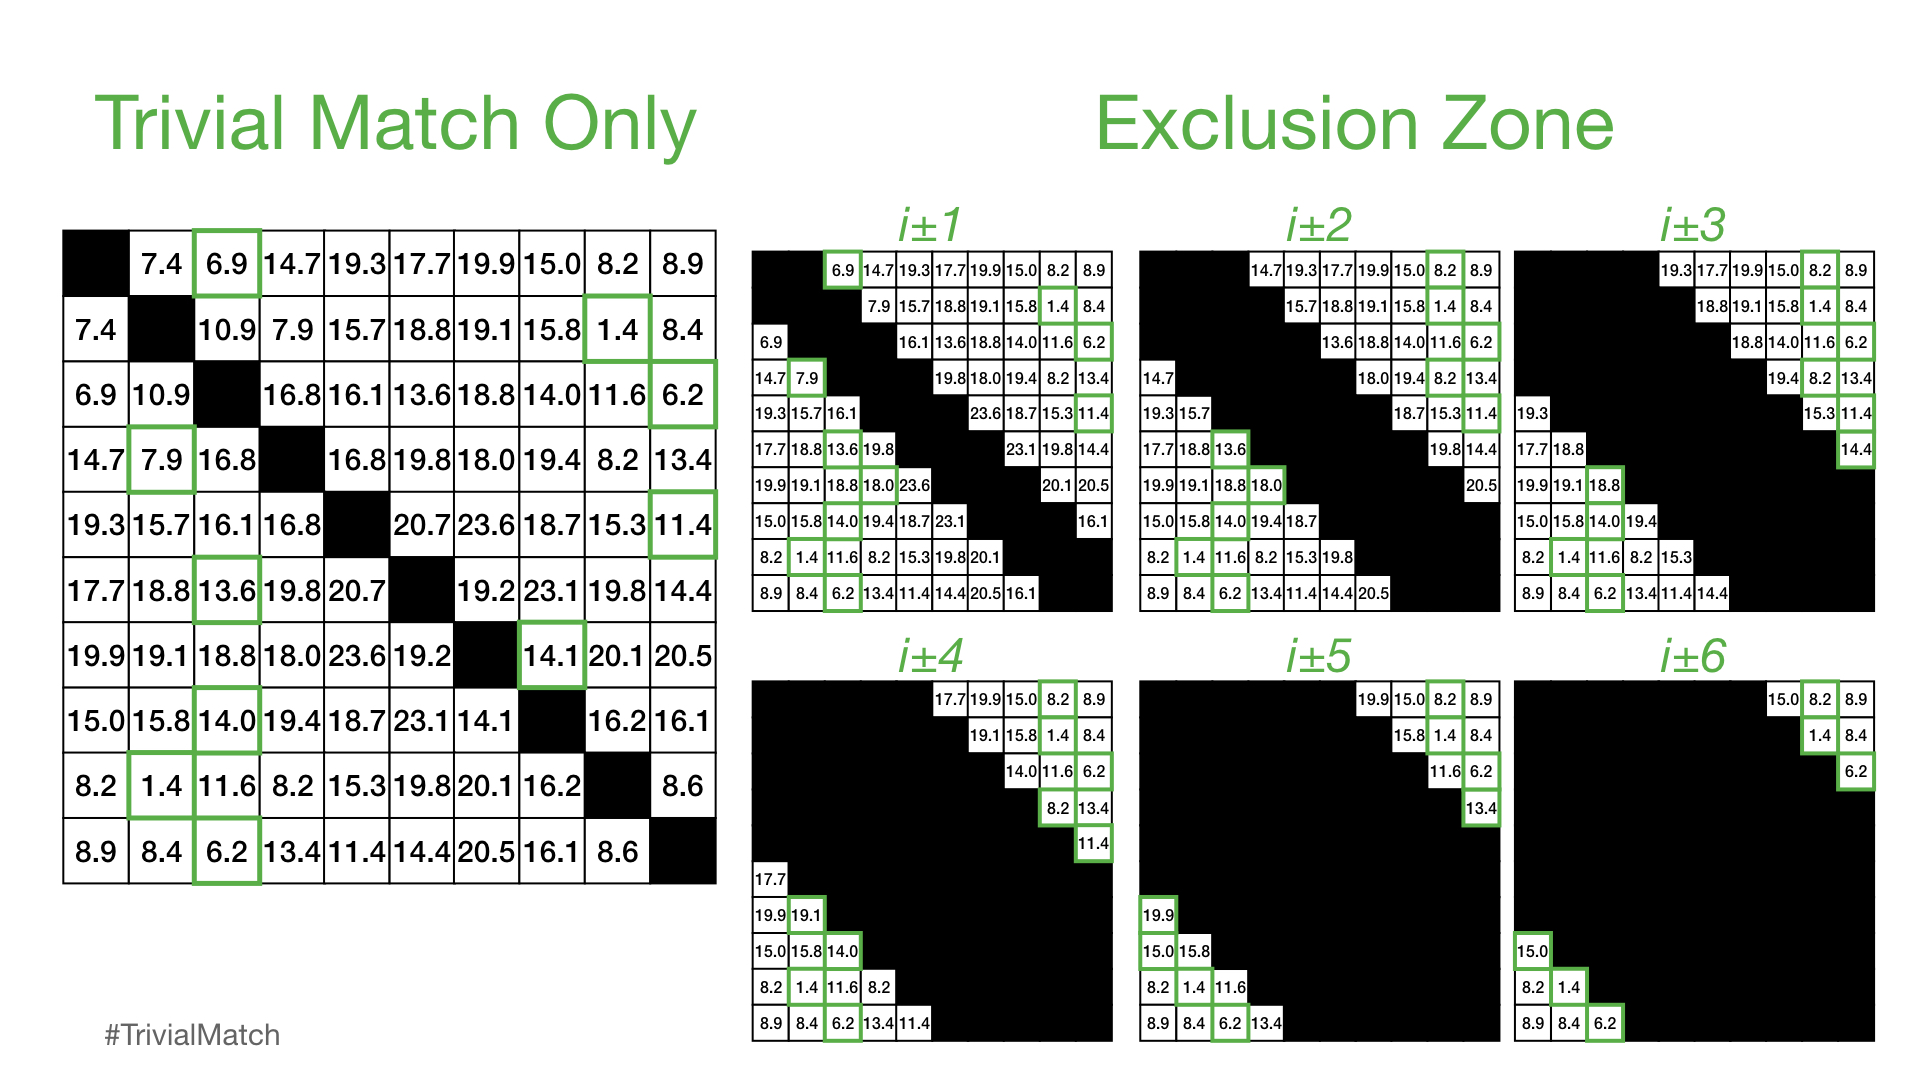
\includegraphics[scale=0.25]{exclusion_zone.jpg}
\caption{Exclusion Zone Sizes}
\label{fig:ExclusionZone}
\end{center}
\end{figure*}

We want to find the nearest neighbor for every subsequence of $T$.  The nearest neighbor information is store in two meta time series, the \emph{Matrix Profile} and the \emph{Matrix Profile Index}:

\textbf{Definition 4:} A \emph{Matrix Profile} $P$ of time series $T$ is a vector of the Euclidean distances between every subsequence of $T$ and its nearest neighbor in $T$.  Formally, $P$ = [min($D_1$), min($D_2$), \ldots{}, min($D_{n-m+1}$)], where $D_i(1 \leq i \leq n-m+1)$ is the distance profile $D_i$ corresponding to the query subsequence $T_{i,m}$ and time series $T$.

The $i^{th}$ element of the Matrix Profile gives the Euclidean distance from the query subsequence $T_{i,m}$ to its nearest neighbor in time series $T$.  However, it does not give the \emph{location} of that nearest neighbor; this information is stored in the \emph{Matrix Profile Index}:

\textbf{Definition 5:} A \emph{Matrix Profile Index} $I$ of time series $T$ is an integer vector: $I = [I_1, I_2, \ldots{}, I_{n-m+1}]$, where $I_i = j$ if $d_{i,j}$ = min($D_i$).

Figure~\ref{fig:DistanceProfilesIntoMatrixProfile} illustrates the relationship between distance profiles and the Matrix Profile.  Each row in the distance matrix is a distance profile.  The minimum of each column is selected and collected in the Matrix Profile.  (The diagonal and the exclusion zone immediately around it are ignored.)  The Matrix Profile Index stores the location where the minimum of that column was found\cite{MatrixProfile14}.

\begin{figure}
\begin{center}
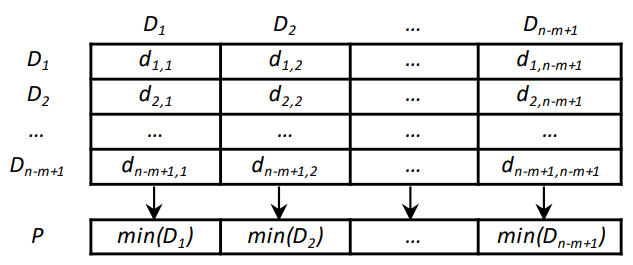
\includegraphics[scale=0.40]{distance_profiles_into_matrix_profile.png}
\caption{Distance Profile Minima Collected into Matrix Profile}
\label{fig:DistanceProfilesIntoMatrixProfile}
\end{center}
\end{figure}

Each distance matrix element $d_{i,j}$ is the distance between $T_{i,m}$ and $T_{j,m} (1 \leq i, j \leq n-m+1)$ of time series $T$.  Figure~\ref{fig:DefinitionsIllustrated} shows an example time series and how the above definitions might be visualized\cite{MatrixProfile11}.  These definitions present the Matrix Profile as a \emph{self-join}.  That is, for every subsequence in a time series $T$, we find its non-trivial-match nearest neighbor within the \emph{same} time series.  To be more broadly useful, the Matrix Profile can be extended to be an AB-join: for every subsequence in a time series $A$, find the nearest neighbors in time series $B$ \cite{MatrixProfile2}\cite{MatrixProfile14}.  For the purposes of this project, we will only deal with the self-join scenario.

\begin{figure}
\begin{center}
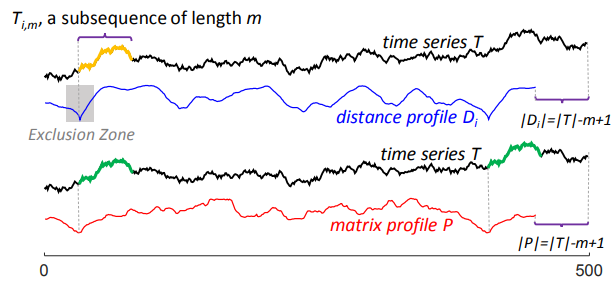
\includegraphics[scale=0.40]{definitions_illustrated.png}
\caption{Definitions Illustrated}
\label{fig:DefinitionsIllustrated}
\end{center}
\end{figure}

\section{Approach}
The Matrix Profile has revolutionized time series data mining tasks and has been heavily optimized, improved, and enhanced since it was announced in 2016.  At the time of this project (2022), there are twenty-three Matrix Profile papers\cite{Keogh} and many Matrix Profile algorithms: STAMP, STAMP\emph{I}, STOMP, SCRIMP, SCRIMP++, SWAMP, and GPU-STOMP.  This project uses the original STAMP algorithm described in the first Matrix Profile paper\cite{MatrixProfile1} with an aim for simplicity in implementation.

The MPI implementation strategy for Matrix Profile is fairly simple for time series data that will fit in the working memory of the MPI processor computers.  
\begin{enumerate}
    \item Leader (rank 0) MPI process parses and validates command line arguments to get an input time series filename, an output matrix profile filename, a subsequence window size, and an input time series column (time series data is frequently stored in comma-separated value formats).
    \item Leader MPI process reads in time series data from the specified input file.
    \item Leader MPI process \texttt{MPI\_Bcast}s time series data to all other processes.
    \item Each MPI process works on distance profile calculations for a segment of time series indices (values of $i$) based on their MPI process rank.  For example, if there are 4 MPI processes, then rank 0 will work on the first fourth of the indices, rank 1 will work on the second fourth of the indices and so forth. 
    \item Each MPI process maintains its own local Matrix Profile and local Matrix Profile Index consisting of the minima and indices of the distance profiles it calculates.  Each time a distance profile is calculated, it is merged into the local Matrix Profile by performing an element-wise minimum with the exception of the trivial match and the surrounding exclusion zone.
    \item After each non-Leader MPI process finishes its segment of time series indices, it \texttt{MPI\_Send}s its local Matrix Profile and local Matrix Profile Index to the Leader (rank 0) process.
    \item After the Leader process finishes its segment of the time series indices, it \texttt{MPI\_Recv}s the local Matrix Profiles and local Matrix Profile Index from the other processes.  For each received local Matrix Profile and local Matrix Profile Index, the Leader process merges the received Matrix Profile and Index into its own using the same element-wise minimum algorithm used to merge a distance profile into the local Matrix Profile.
    \item Once all the other processes' local Matrix Profiles and Indices have been merged, the Leader process writes the final Matrix Profile to the output file.
\end{enumerate}

\section{Simulation}
There are no simulations for this project.

\section{Tests}
In order to validate the finished MPI implementation of Matrix Profile in C++ a test suite was created.  The test suite currently consists of nine input time series and their corresponding matrix profiles.  The STUMPY\cite{Stumpy} Python library implementation of the Matrix Profile was used to process the input time series and the output Matrix Profile data structures were captured.  The MPI Matrix Profile implementation will be validated as correct if the output Matrix Profile data structures match those created by the STUMPY Matrix Profile implementation. 

Additionally, unit tests are being created to validate that each component of the MPI Matrix Profile implementation works as expected.  We are also utilizing GitHub Actions to perform  multi-platform (Linux, MacOS, and Windows) builds and unit tests before pull requests are allowed to merge into the \texttt{main} branch.  See https://github.com/rmcnew/parallel\_group\_project/actions for more information.


\section{Preliminary Results}
At this time we do not have any preliminary results.  


% ** Should the task lists and burndown charts be grouped like this or should
% ** we place the task list and burndown chart together by sprint, that is,
% ** Sprint 1 task list and burndown chart, Sprint 2 task list and burndown chart, etc.  ?

\section{CPU Graph}

Figure~\ref{fig:CPU Graph} Shows the CPU usage percentage. 100% means 1 core, 300% means 3 cores were used.

\begin{figure*}
\begin{center}
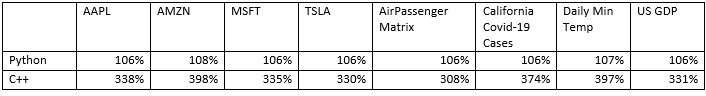
\includegraphics[scale=1.05]{CPU.png}
\caption{CPU usage percentage. 100% means 1 core, 300% means 3 cores were used.}
\label{fig:CPU Usage}
\end{center}
\end{figure*}

\section{Time Graph}

Figure~\ref{fig:Time Graph} Shows the how many seconds it took the Python and C++ code to complete time series.

\begin{figure*}
\begin{center}
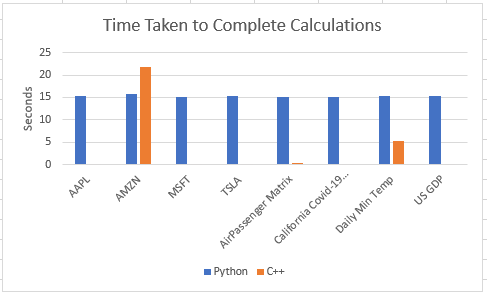
\includegraphics[scale=1.05]{Time.png}
\caption{Compares how many seconds it took the Python code and C++ code to complete time series calculations}
\label{fig:Time to complete time series}
\end{center}
\end{figure*}

\section{CPU Graph}

Figure~\ref{fig:CPU Graph} Shows the CPU usage percentage. 100% means 1 core, 300% means 3 cores were used.

\begin{figure*}
\begin{center}
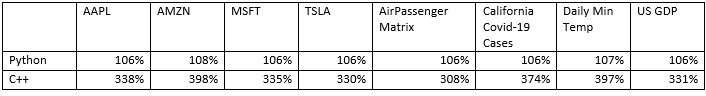
\includegraphics[scale=1.05]{CPU.png}
\caption{CPU usage percentage. 100% means 1 core, 300% means 3 cores were used.}
\label{fig:CPU Usage}
\end{center}
\end{figure*}

\section{Memory Graph}

Figure~\ref{fig:Memory Graph} Shows the amount of kilobytes that the Python and C++ programs used.

\begin{figure*}
\begin{center}
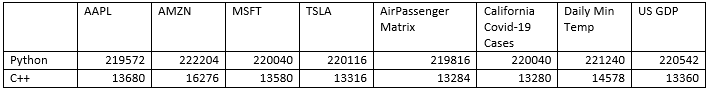
\includegraphics[scale=1.05]{Memory.png}
\caption{The amount of kilobytes the Python and C++ programs used.}
\label{fig:Memory Usage}
\end{center}
\end{figure*}

\section{Sprint Tasks}

Figure~\ref{fig:SprintTasks} gives the list of tasks performed thus far, who completed the task, and the number of Story Points for that task.

\begin{figure*}
\begin{center}
\includegraphics[scale=1.05]{AllTasks.png}
\caption{List of tasks, who completed the task and number of Story Points}
\label{fig:SprintTasks}
\end{center}
\end{figure*}


\section{Burndown Chart}

Figure~\ref{fig:BurndownChart} shows a burndown chart for the sprints.

\begin{figure*}
\begin{center}
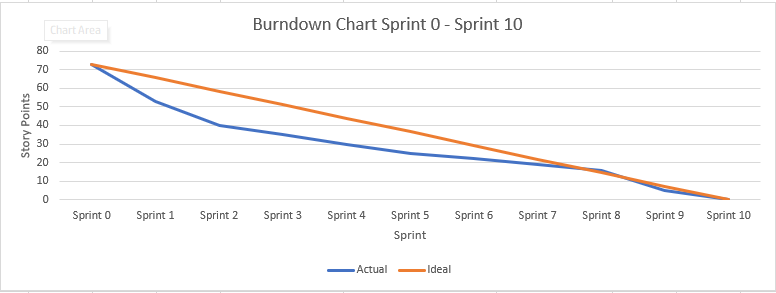
\includegraphics[scale=1.05]{Burndown.png}
\caption{Burndown chart from Sprint 0 to Sprint 10}
\label{fig:BurndownChart}
\end{center}
\end{figure*}


\bibliographystyle{IEEEtran}

% number is the number of reference labels
\begin{thebibliography}{7}  

\bibitem{MatrixProfile1} C. M. Yeh et al., "Matrix Profile I: All Pairs Similarity Joins for Time Series: A Unifying View That Includes Motifs, Discords and Shapelets," 2016 IEEE 16th International Conference on Data Mining (ICDM), 2016, pp. 1317-1322, doi: 10.1109/ICDM.2016.0179.

\bibitem{MatrixProfile2} Y. Zhu et al., "Matrix Profile II: Exploiting a Novel Algorithm and GPUs to Break the One Hundred Million Barrier for Time Series Motifs and Joins," 2016 IEEE 16th International Conference on Data Mining (ICDM), 2016, pp. 739-748, doi: 10.1109/ICDM.2016.0085.

\bibitem{MatrixProfile11} Y. Zhu et al., "Matrix Profile XI: SCRIMP++: Time Series Motif Discovery at Interactive Speeds," 2018 IEEE International Conference on Data Mining (ICDM), 2018, pp. 837-846, doi: 10.1109/ICDM.2018.00099.

\bibitem{MatrixProfile14} Z. Zimmerman et al., "Matrix Profile XIV: Scaling Time Series Motif Discovery with GPUs to Break a Quintillion Pairwise Comparisons a Day and Beyond," 2019 ACM Symposium, pp. 74-86. doi: 10.1145/3357223.3362721. 

\bibitem{DynamicTimeWarping} T. Rakthanmanon et al., "Searching and Mining Trillions of Time Series Subsequences under Dynamic Time Warping," In Proceedings of the 18th ACM SIGKDD international conference on Knowledge discovery and data mining (KDD '12). 2012. Association for Computing Machinery, New York, NY, USA, 262–270. DOI:https://doi.org/10.1145/2339530.2339576.

\bibitem{Stumpy} S.M. Law, (2019). "STUMPY: A Powerful and Scalable Python Library for Time Series Data Mining," Journal of Open Source Software, 4(39), 1504. [Online]. Available: https://github.com/TDAmeritrade/stumpy.

\bibitem{Keogh} E. Keogh, \emph{The UCR Matrix Profile Page}, 2021. [Online]. Available: https://www.cs.ucr.edu/~eamonn/MatrixProfile.html.


\end{thebibliography}

\end{document}
